\chapter{Efficient Encoding, Decoding, and Indexing} \label{chap:coding}


\section{SDOG}
In order to identify and distinguish the cells of a grid, there needs to be a method to assign a unique index to each cell.
A good indexing scheme will allow for efficient data insertion, retrieval, and manipulation via a set of queries.
Examples of some of these queries are: point to cell, which give the index of the cell containing a given point; index inversion, which calculates a cell's location and geometry from the index; neighbourhood queries; and in the case of a hierarchical grid, hierarchy traversal to find parent and children cells.


Due to the fact that SDOG refinement is based on the midpoints of spherical coordinates, an indexing scheme that is efficient for many of the above operations can be easily developed.
At any refinement level, $k$, each cell can be given an integer index in each spherical coordinate ranging from zero to $2^{k} - 1$.
To address the degenerate refinement of certain cells, these integer indices are modified appropriately with divisions by powers of two, which can be done quickly with bit shift operations.
The integer indices can then be linearized by various methods, one good choice being a Z-order curve \cite{morton1966computer} as used in \cite{yu2009sdog}.


A more detailed description of degenerate Z-order indexing for SDOG grids, including algorithms for point to cell and index inversion operations, can be found in \cite{yu2009coding}.
Explain SDOG indexing.
Modified Morton based.
Conventional algorithms are hierarchical (linear on k).
We derive direct index versions (constant on k).


All algorithms provided operate on a standard octant. For full SDOG implementations, pre and post operations needed.
Encoding. Pre: convert coordinates to standard octant. Post: prepend leading bit and octant code
Decoding. Pre: get k and convert coordinates to standard octant. Post: convert output to coordinates of actual octant


\subsection{Encoding Algorithms}
Below provide hierarchal algorithm and our new one.
Then we compare runtime.


\subsubsection{Hierarchical}
Provide pseudo code here. Algorithm~\ref{alg:encode}. Input is a point $p$ after going through pre and refinement level $k$. Output is index $i$ to feed into post.


\begin{algorithm}
	\caption{Hierarchical point encoding for SDOG}
	
	\begin{algorithmic}
		
		\STATE cellBoundaries $\leftarrow$ boundaries of octant
		\STATE currCellType $\leftarrow$ SG
		\STATE $i \leftarrow 0$
		
		\FOR{$k$ iterations}
			\STATE use refinement rules for currCellType with cellBoundaries to find child cells
			\STATE determine which child contains $p$
			\STATE cellBoundaries $\leftarrow$ boundaries of child
			\STATE currCellType $\leftarrow$ type of child
			\STATE $i \leftarrow \operatorname{append}(i, \mathrm{child~index})$
		\ENDFOR
		\RETURN $i$
		 
	\end{algorithmic}
	\label{alg:encode}
\end{algorithm}


\subsubsection{Direct}

\begin{equation*}
\hat{r} = \frac{r}{R_\mathrm{max}}
\end{equation*}

\begin{equation*}
\hat{\varphi} = \frac{2 \varphi}{\pi}
\end{equation*}

\begin{equation*}
\hat{\lambda} = \frac{2 \lambda}{\pi}
\end{equation*}

\begin{equation*}
s = \lfloor \log_{0.5} \hat{r} \rfloor
\end{equation*}

\begin{equation*}
z = \lfloor \log_{0.5} ( 1 - \hat{\varphi} ) \rfloor
\end{equation*}

\begin{equation*}
k_\varphi = \min ( s, k )
\end{equation*}

\begin{equation*}
k_\lambda = \min ( k_\varphi + z, k )
\end{equation*}

\begin{equation*}
r_i = 2^k \cdot ( 1 - \hat{r} )
\end{equation*}

\begin{equation*}
\varphi_i = 2^{k - k_\varphi} \cdot \hat{\varphi}
\end{equation*}

\begin{equation*}
\lambda_i = 2^{k - k_\lambda} \cdot \hat{\lambda}
\end{equation*}

\begin{equation*}
i = \operatorname{Morton}( \lambda_i, \varphi_i, r_i ) + 2^{3k}
\end{equation*}


\subsubsection{Runtime Comparison}


\begin{figure}[htp!]
	\centering
	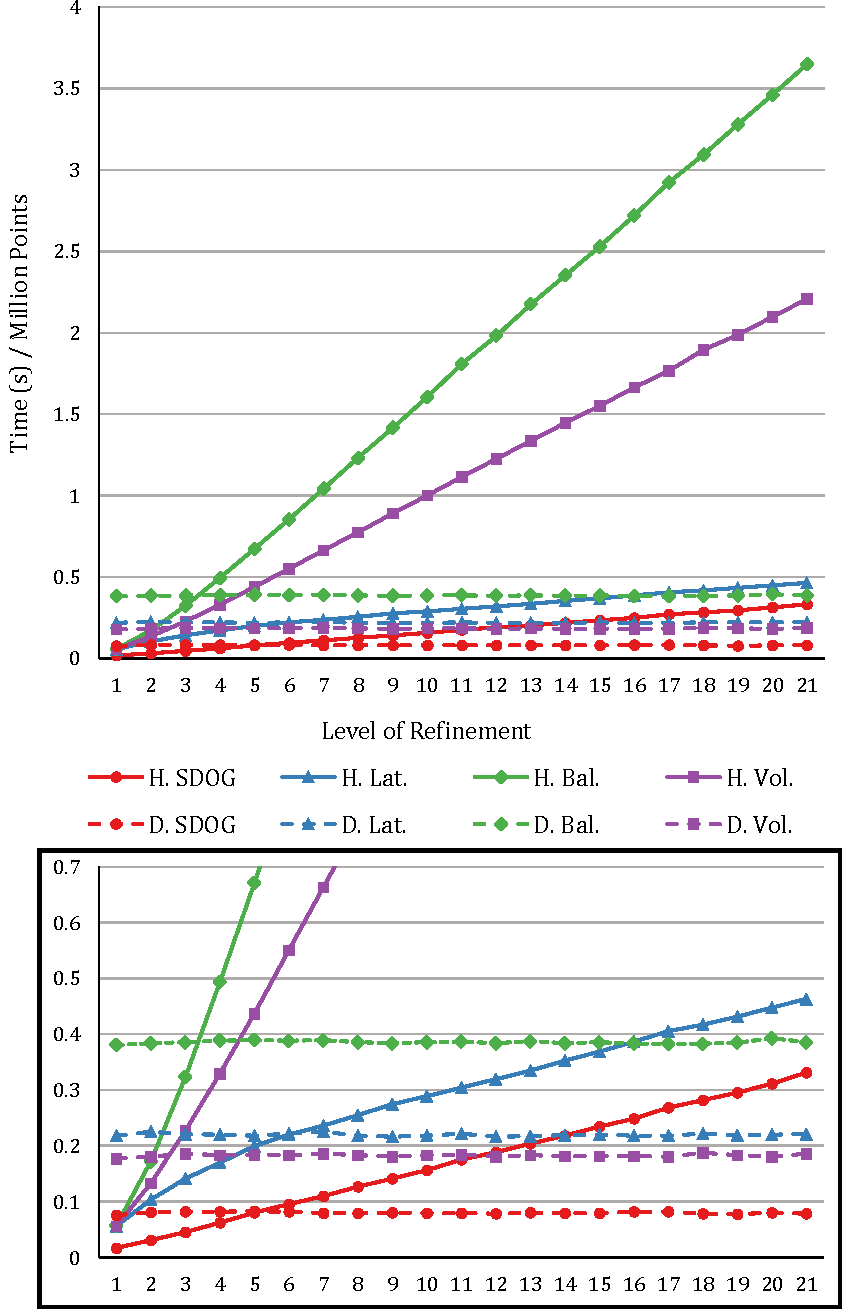
\includegraphics[width=0.8\textwidth]{point-to-index.pdf}
	\caption[Runtime comparison of SDOG point encoding algorithms]{
		A caption will go here.
		The caption may be long.
		This is text that is filling space so that this placeholder caption is longer than if the text was not here.
		Caption caption caption.
		Now the text will repeat...
		A caption will go here.
		The caption may be long.
	}
	\label{fig:point-to-index}
\end{figure}


\subsection{Decoding Algorithms}
Below provide hierarchal algorithm and our new one.
Then we compare runtime.


\subsubsection{Hierarchical}
Provide pseudo code here.
Algorithm~\ref{alg:decode}. Input is an index $i$ after going through pre-operations (so also $k$). Output is index cell boundaries to go into post.


\begin{algorithm}
	\caption{Hierarchical cell decoding for SDOG}
	
	\begin{algorithmic}
		
		\STATE cellBoundaries $\leftarrow$ boundaries of octant
		\STATE currCellType $\leftarrow$ SG
		
		\FOR{$k$ iterations}
			\STATE use refinement rules for currCellType with cellBoundaries to find child cells
			\STATE $c \leftarrow$ highest three bits of $i$
			\STATE remove highest three bits of $i$
			\STATE determine which child cell matches $c$
			\STATE cellBoundaries $\leftarrow$ boundaries of $c$
			\STATE currCellType $\leftarrow$ type of $c$
		\ENDFOR
		\RETURN cellBoundaries
		
	\end{algorithmic}
	\label{alg:decode}
\end{algorithm}


\subsubsection{Direct}

%\begin{equation*}
%k = \left\lfloor \frac{ \log_{2}i}{3} \right\rfloor
%\end{equation*}

\begin{equation*}
( \lambda_i, \varphi_i, r_i ) = \operatorname{Morton}^{-1} (i)% \oplus 2^{3k})
\end{equation*}

\begin{equation*}
\hat{r}_\mathrm{max} = 1 - \frac{r_i}{2^k}
\end{equation*}

\begin{equation*}
\hat{r}_\mathrm{min} = 1 - \frac{r_i + 1}{2^k}
\end{equation*}

\begin{equation*}
s = \lfloor \log_{0.5} \hat{r}_\mathrm{max} \rfloor
\end{equation*}

\begin{equation*}
k_\varphi = \min ( s, k )
\end{equation*}

\begin{equation*}
\hat{\varphi}_\mathrm{max} = \frac{\varphi_i + 1}{2^{k - k_\varphi}}
\end{equation*}

\begin{equation*}
\hat{\varphi}_\mathrm{min} = \frac{\varphi_i}{2^{k - k_\varphi}}
\end{equation*}

\begin{equation*}
z = \lfloor \log_{0.5} ( 1 - \hat{\varphi}_\mathrm{min} ) \rfloor
\end{equation*}

\begin{equation*}
k_\lambda = \min ( k_\varphi + z, k )
\end{equation*}

\begin{equation*}
\hat{\lambda}_\mathrm{max} = \frac{\lambda_i + 1}{2^{k - k_\lambda}}
\end{equation*}

\begin{equation*}
\hat{\lambda}_\mathrm{min} = \frac{\lambda_i}{2^{k - k_\lambda}}
\end{equation*}


\subsubsection{Runtime Comparison}


\begin{figure}[htp!]
	\centering
	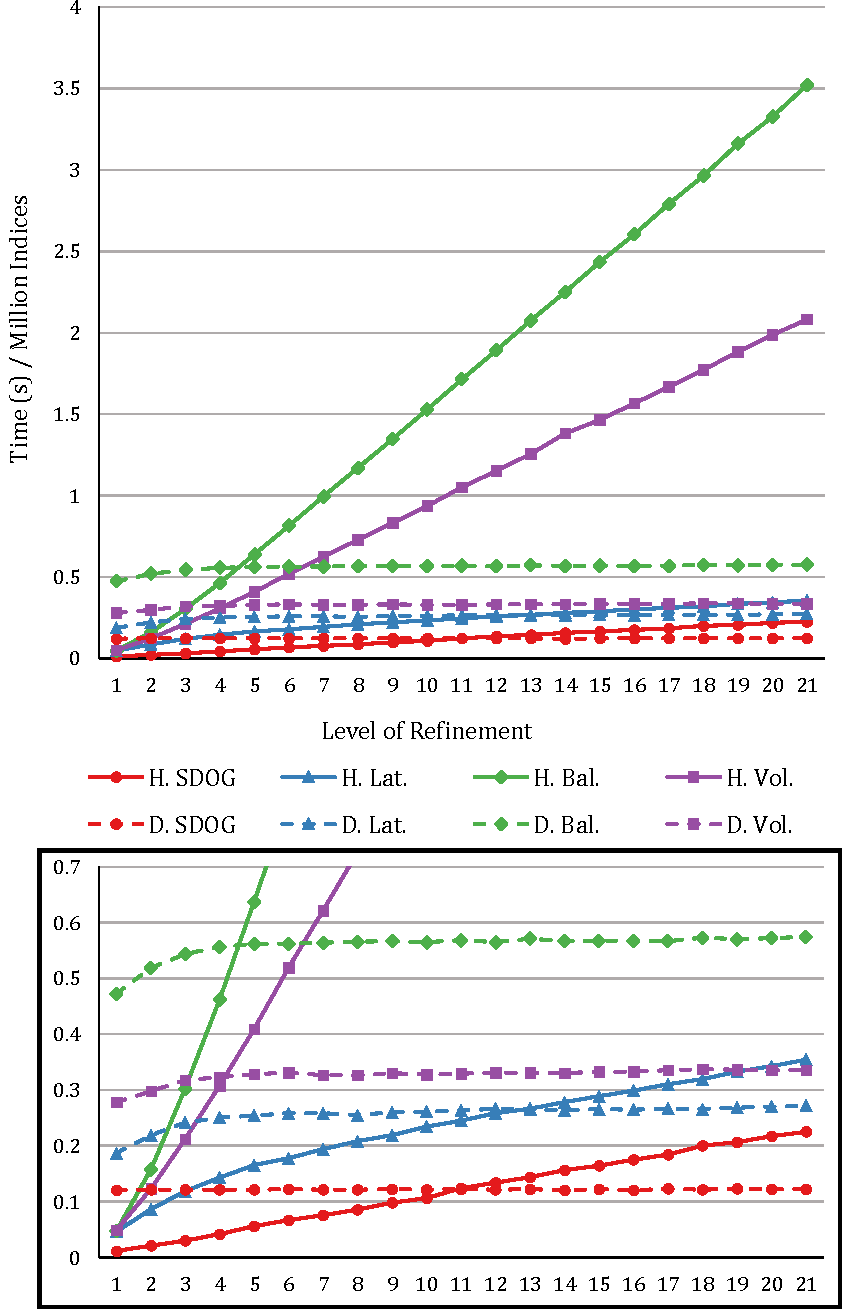
\includegraphics[width=0.8\textwidth]{index-to-range.pdf}
	\caption[Runtime comparison of SDOG decoding algorithms]{
		A caption will go here.
		The caption may be long.
		This is text that is filling space so that this placeholder caption is longer than if the text was not here.
		Caption caption caption.
		Now the text will repeat...
		A caption will go here.
		The caption may be long.
	}
	\label{fig:index-to-range}
\end{figure}


\subsection{Indexing Operations}
Indexing stuff here I guess?
Neighbours are tricky...


\section{Extension Method}


\subsection{Encoding Algorithm}


\subsection{Decoding Algorithm}


\subsection{Indexing Operations}
An important component of a conventional DGGS is the indexing scheme for cells.
Indices in a DGGS are used to not only identify and linearize cells but also as a means of navigating the grid for various spatial queries~\cite{alderson2020digital}.
To this end, it is important to be able to perform certain operations on said indices efficiently.
The most fundamental of these operations are parent queries, which return the parent (or with non-congruent refinement, \textit{parents}) of a given cell; child queries, which return the children of the cell; and neighbour queries, which return cells that share an edge (or in 3D a face) with the cell.
These operations serve as the building blocks for more complex geospatial queries done with the grid system, such as region growing, data convolution and correlation, feature rasterization, and buffering.
Because of this, creating suitable indexing for a 3D DGGS is an essential task.


With our method---similar to encoding and decoding---we define these operations in terms of surface and radial components.
This split not only simplifies the problem of indexing but also ensures the 3D indexing is consistent with that of the input DGGS.
Referring back to Figures~\ref{fig:indexing} and \ref{fig:3d-coding}, we let $i_s$ be the surface index of a cell and $i_\ell$ be the layer index.
For each of these components, we assume there is a corresponding parent, child, and neighbour operation.
For the surface index, this comes directly from the input DGGS indexing, whereas for the layer index, these would need to be defined.
Using the component operations, we define the corresponding 3D operations as follows.


\paragraph{Parents}
The parent(s) of a cell depend on if the layer of the cell and its parent layer have the same, or different, values of $k_s$.
Let $i_\ell' = \operatorname{parent}(i_\ell)$; if the value of $k_s$ is the same, then the single parent is simply $(i_s, i_\ell')$.
In most cases, the value of $k_s$ for $i_\ell'$ is some number $m$ (often one, but not always) less than that of $i_\ell$.
In this case, the parent(s) are given by $\operatorname{parents}^m(i_s) \times i_\ell$.


\paragraph{Children} The children of a cell depend on if the cell belongs to a central or normal layer.
For normal layers, the set of children is simply $\operatorname{children}(i_s) \times \operatorname{children}(i_\ell)$.
For central layers, the child who belongs to the new central layer must be distinguished from the other child layer(s).
Call the index of the new central layer $c_\ell$; then, this child is given by $(i_s, c_\ell)$.
Let $ N_\ell$ give the set of the other children layer indices (normal layers).
These layers have the surface refinement applied $w$ times, so the resulting children are $\operatorname{children}^w(i_s) \times N_\ell$


\paragraph{Neighbours} We split neighbours into three categories: neighbours in the same layers as the cell, neighbours in the layer above the cell, and neighbours in the layer below the cell.
If a cell belongs to the outermost or innermost (central) layer, then it will not have neighbours in the layer above or below, respectively.
Neighbours in the same layer are simply $\operatorname{neighbours}(i_s) \times i_\ell$.
Let $i_\ell^+$ be the layer above $i_\ell$ and $i_\ell^-$ be the layer below.
If $i_\ell^+$ has the same value of $k_s$ as $i_\ell$, then the single neighbour above is $(i_s, i_\ell^+)$.
In the other case, where the value of $k_s$ for $i_\ell^+$ is some number $m$ greater than that of $i_\ell$, the neighbours are given by $\operatorname{children}^m(i_s) \times i_\ell^+$.
Likewise, if $i_\ell^-$ has the same value of $k_s$ as $i_\ell$, there is one neighbour below given by $(i_s, i_\ell^-)$.
In the case that the value of $k_s$ for $i_\ell^-$ is some number $m$ less than that of $i_\ell$, the neighbours are given by $\operatorname{parents}^m(i_s) \times i_\ell^-$

\section{Summary}